% +------------------------------------------------------------------------+
% | Reference manual page: intro.tex
% +------------------------------------------------------------------------+
% | 09.02.2006   Marc Pouget and Fr�d�ric Cazals
% | Package: Jet_fitting_3
% | 
\RCSdef{\RCSintroRev}{$Id$}
\RCSdefDate{\RCSintroDate}{$Date$}
% |
%%RefPage: end of header, begin of main body
% +------------------------------------------------------------------------+

\ccRefChapter{Estimation of Local Differential Properties of Sampled
Surfaces via Polynomial Fitting\label{ref_chap:Jet_fitting_3}}
  
\ccChapterAuthor{Marc Pouget \and Fr\'ed\'eric Cazals}

%\subsection*{Introduction}

%The following picture illustrates the template dependencies.
%\begin{figure}[h!]
%\begin{ccTexOnly}
%\centerline{
%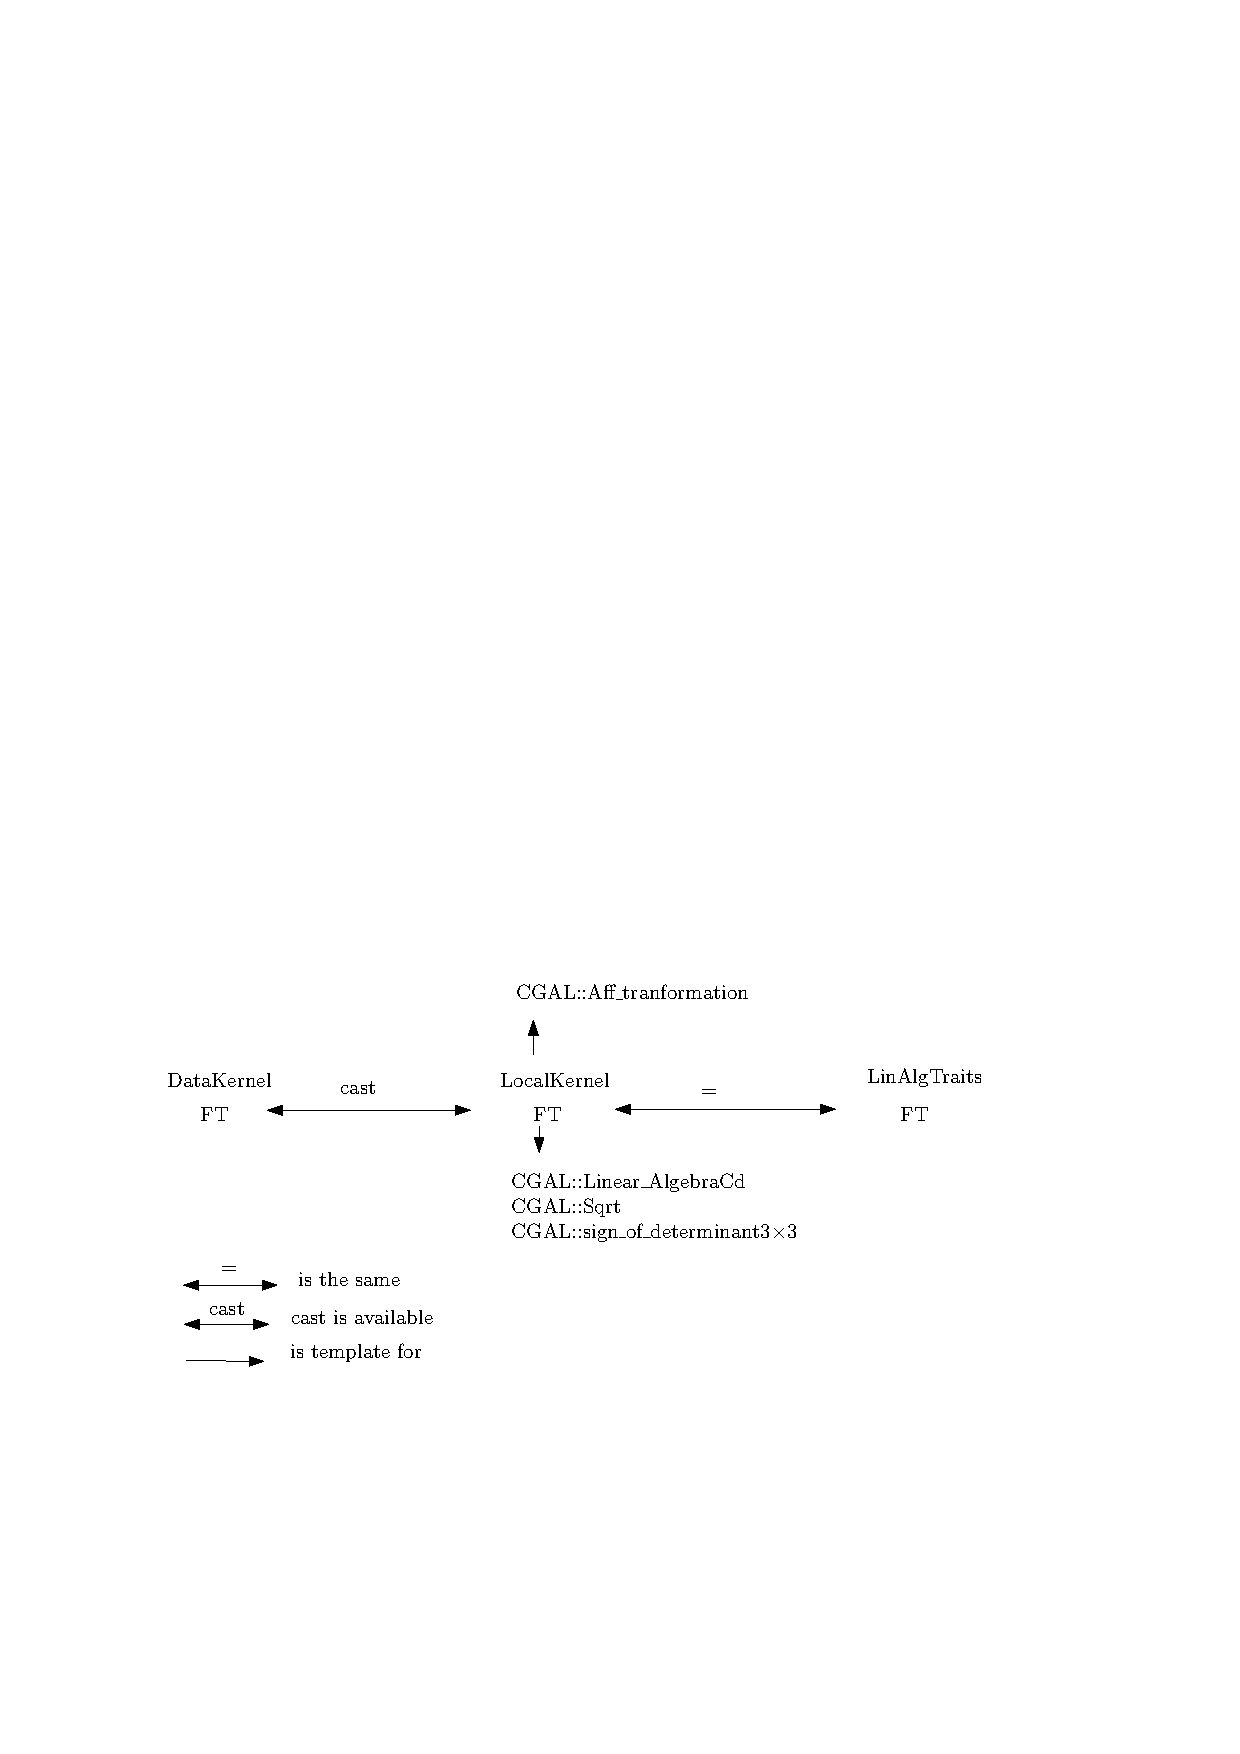
\includegraphics[width=.5\linewidth]{Jet_fitting_3_ref/template_dependence}}
%\end{ccTexOnly}

%\label{fig:template_dependence}
%\caption{}

%\begin{ccHtmlOnly}
%<CENTER>
%<img border=0 src="template_dependence.jpg" width=600>
%</CENTER>
%\end{ccHtmlOnly}
%\end{figure}


\ccRequirements

\subsection*{Concepts}
\ccRefConceptPage{DataKernel} \\
\ccRefConceptPage{LocalKernel} \\
\ccRefConceptPage{SvdTraits} \\

\subsection*{Classes}
\ccRefIdfierPage{CGAL::Monge_via_jet_fitting< DataKernel, LocalKernel, SvdTraits>::Monge_form}\\
\ccRefIdfierPage{CGAL::Monge_via_jet_fitting<DataKernel, LocalKernel, SvdTraits>}\\
\ccRefIdfierPage{CGAL::Eigen_svd}\\
\ccRefIdfierPage{CGAL::Lapack_svd}\\

\subsection*{Global Functions}
The insert operator (\ccc{operator<<} )  is overloaded for the class
\ccc{Monge_form}.

% +------------------------------------------------------------------------+
%%RefPage: end of main body, begin of footer
% EOF
% +------------------------------------------------------------------------+

